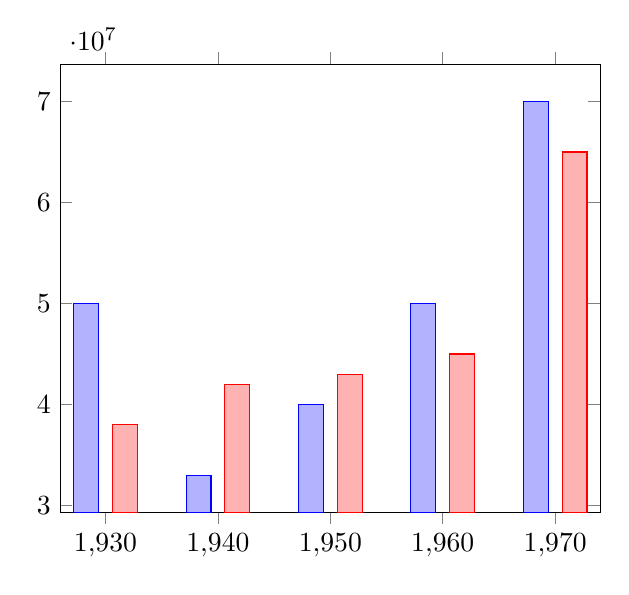
\begin{tikzpicture} \begin{axis}[
    %x tick label style={
    %    /pgf/number format/1000 sep=},
    %ylabel=Population, enlargelimits=0.15,
    %legend style={at={(0.5,-0.15)},
    %anchor=north,legend columns=-1}, 
    ybar=5pt,bar width=9pt,
    %nodes near coords,point meta=y *10^-7, % the displayed number
    ]
    \addplot coordinates {
        (1930,50e6) (1940,33e6)
        (1950,40e6) (1960,50e6) (1970,70e6)
    };
    \addplot coordinates {
        (1930,38e6) (1940,42e6)
        (1950,43e6) (1960,45e6) (1970,65e6)};
\end{axis}
\end{tikzpicture}
